\chapter{Risultati}
\label{ch:risultati}

In questo capitolo verranno presentati i risultati ottenuti durante la fase di
benchmarking della libreria nella procedura \textit{gain}, ovvero quella
ottimizzata. Questa fase è di notevole importanza, in quanto permette di
valutare il lavoro svolto, confrontando tutte le implementazioni tra loro, oltre
all'implementazione originale, per avere un quadro completo della situazione finale.

\section{Metodologia di valutazione}
\label{sec:bencharmking}

Per poter valutare le prestazioni della libreria, sono stati eseguiti diversi test di benchmarking,
che hanno permesso di confrontare le diverse implementazioni tra loro. Inoltre,
è stato fondamentale valutare la correttezza matematica della procedura
modificata, per garantire che non siano stati introdotti errori durante la fase di
programmazione, per tutti e tre i framework di parallelizzazione. In merito allo
svolgimento, la liberia \textit{CoopeRIS} è dotata di un set di \textit{unit
test}, che sono stati eseguiti durante la fase di sviluppo. Tutte le misurazioni
sono state eseguite su macchine con diverse configurazioni hardware, per poter
valutare le prestazioni in diversi scenari.

\section{Benchmarking della libreria}
\label{sec:benchmarking}

Il benchmarking della procedura ottimizzata e della libreria è stato eseguito
senza la necessità di alcuno dei framework esterni citati nel capitolo
\ref{subsec:risframework}. Questo è stato essenziale per poter valutare le prestazioni
della libreria in modo puro e indipendente. Per fare ciò, è stato creato un programma
molto semplice, che ha eseguito ripetutamente le procedure sotto esame, misurando
il tempo di esecuzione di ciascuna di esse. Il programma è stato eseguito su
diverse macchine, soprattutto per
poter valutare situazioni con un elevato numero di core CPU. Per garantire una maggiore
precisione, ciascuna misurazione è stata eseguita più volte, da un minimo di dieci
fino ad un massimo di mille, per calcolarne la media ed eliminare eventuali
errori dovuti a fluttuazioni dell'ambiente di esecuzione.

\subsection{Risultati complessivi}
\label{subsec:risultati-complessivi}

I risultati complessivi del benchmarking della libreria sulla procedura \textit{gain}
sono stati molto positivi. Le ottimizzazioni apportate hanno ottenuto un notevole
incremento prestazionale, raggiungendo in alcuni casi un incremento di
prestazioni fino a due ordini di grandezza nei casi in cui le RISs contenevano
il numero massimo di elementi supportati. Questo dimostra totalmente l'efficacia
delle ottimizzazioni apportate.

\begin{figure}[!ht]
  \centering
  \subfloat[
  \centering
  scala lineare]{{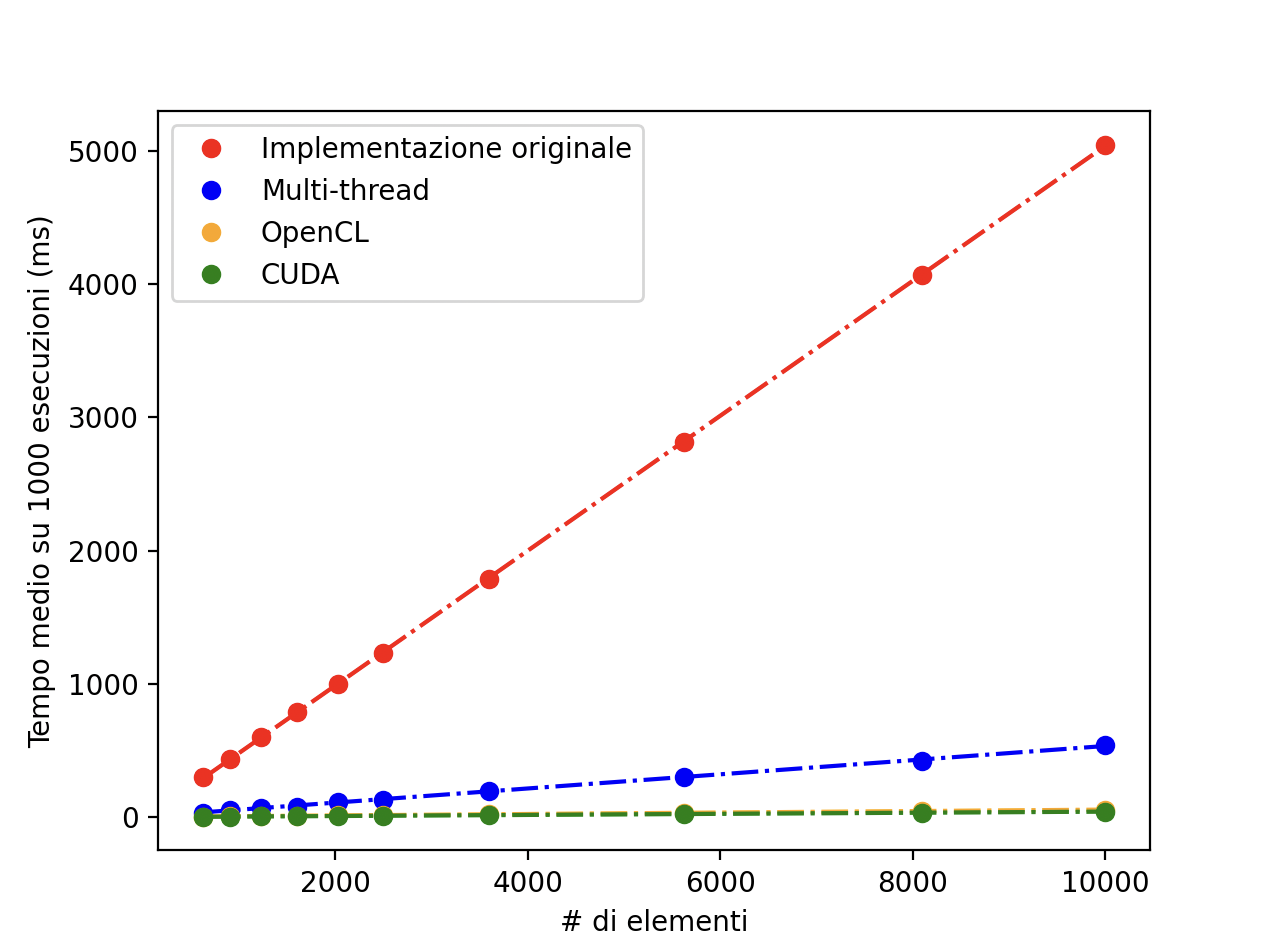
\includegraphics[width=8cm]{images/results/gain-over-elem.png}\label{fig:risultati-complessivi}}}
  \subfloat[
  \centering
  scala logaritmica]{{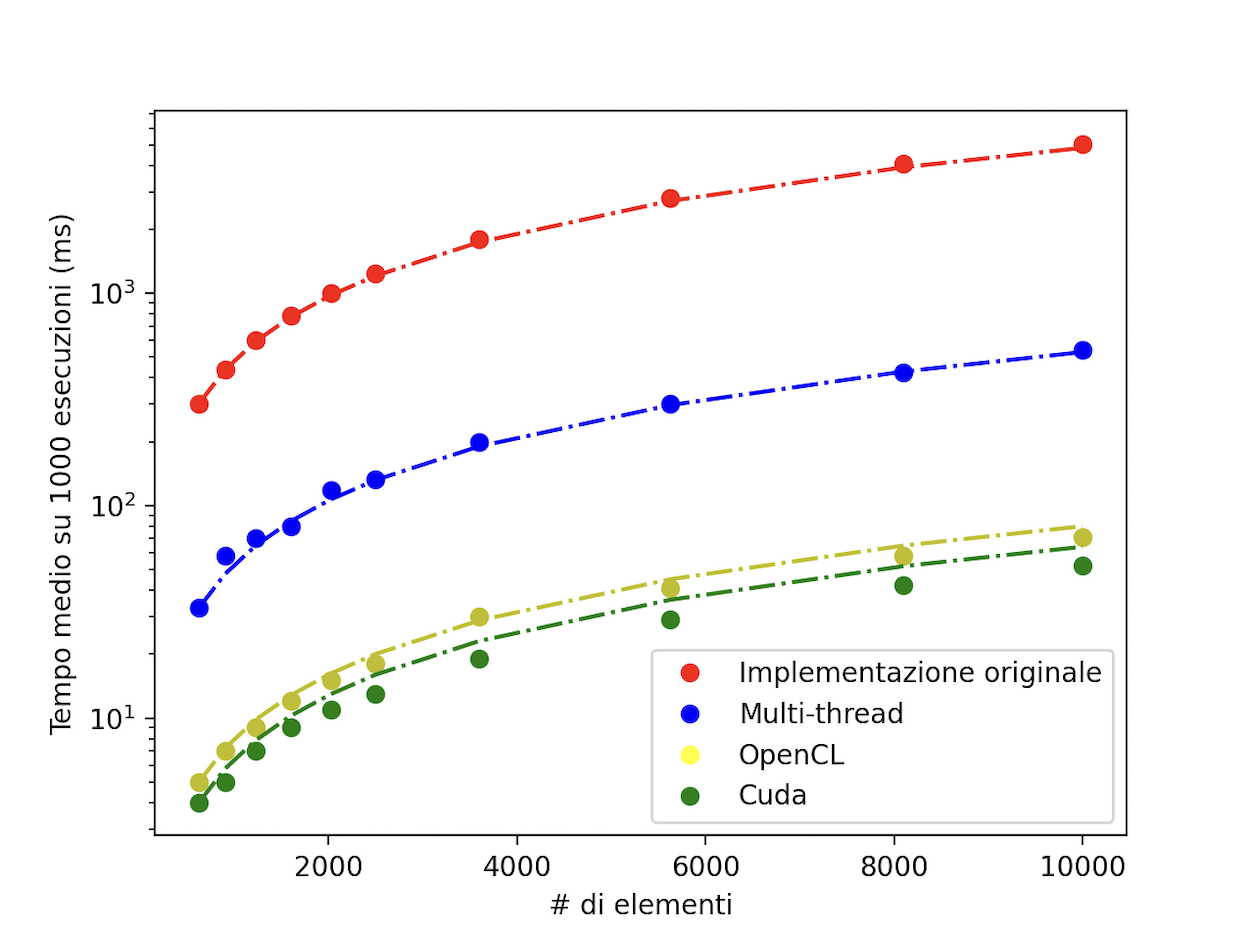
\includegraphics[width=8cm]{images/results/log-gain-over-elem.png}\label{fig:risultati-complessivi-log}}}
  \caption{Risultati complessivi del benchmarking}
\end{figure}

Nelle figure \ref{fig:risultati-complessivi} e
\ref{fig:risultati-complessivi-log} sono riportati i risultati complessivi del
benchmarking della libreria. La linea tratteggiata rappresenta il tempo di esecuzione
ideale, calcolato come il tempo della procedura sul tempo con minor numero di
elementi moltiplicato per ogni successivo numero di elementi. I punti invece rappresentano
rispettivamente i tempi di esecuzione della procedura non ottimizzata e della procedura
ottimizzata tramite multi-threading, OpenCL e CUDA. In figura \ref{fig:risultati-complessivi-log}
sono riportati i risultati in scala logaritmica, per migliorare la leggibilità
dei dati, soprattutto nei casi delle implementazioni tramite GPU.

\subsection{Risultati: CPU single-thread vs multi-thread}
\label{subsec:risultati-cpu}

Particolare attenzione è stata posta nel confronto tra l'implementazione
originale e multi-thread della procedura \textit{gain}. Molteplici test e
benchmark sono stati eseguiti per valutare le prestazioni con diversi numeri di
thread CPU. In figura \ref{fig:risultati-cpu} sono riportati i risultati ottenuti
al variare del numero di thread utilizzati, per quattro delle configurazioni di
elementi RISs. Si evince chiaramente come l'implementazione multi-thread, ad un
numero di thread molto elevato, saturi le prestazioni della CPU e non permetta di
ottenere ulteriori incrementi prestazionali, dovuto al crescente aumento lineare
di overhead necessario all'avvio e sincronizzazione di tutti i thread. Si noti inoltre
come, superata la soglia dei \textit{65} thread, si verifichi un fenomeno dove l'aggiunta
di un thread che necessariamente deve essere eseguito tramite \textit{hyperthreading},
riduca la performance generale della procedura. Invece, in figura
\ref{fig:jobs-per-thread} è riportato il confronto tra la grandezza dei dati da
elaborare per thread, al variare del numero di thread utilizzati. Si ritrovano
anche qui lo stesso fenomeno di diminuzione delle prestazioni dovuto all'\textit{hyperthreading}.

\begin{figure}[!ht]
  \begin{minipage}[t]{0.5\linewidth}
    \centering
    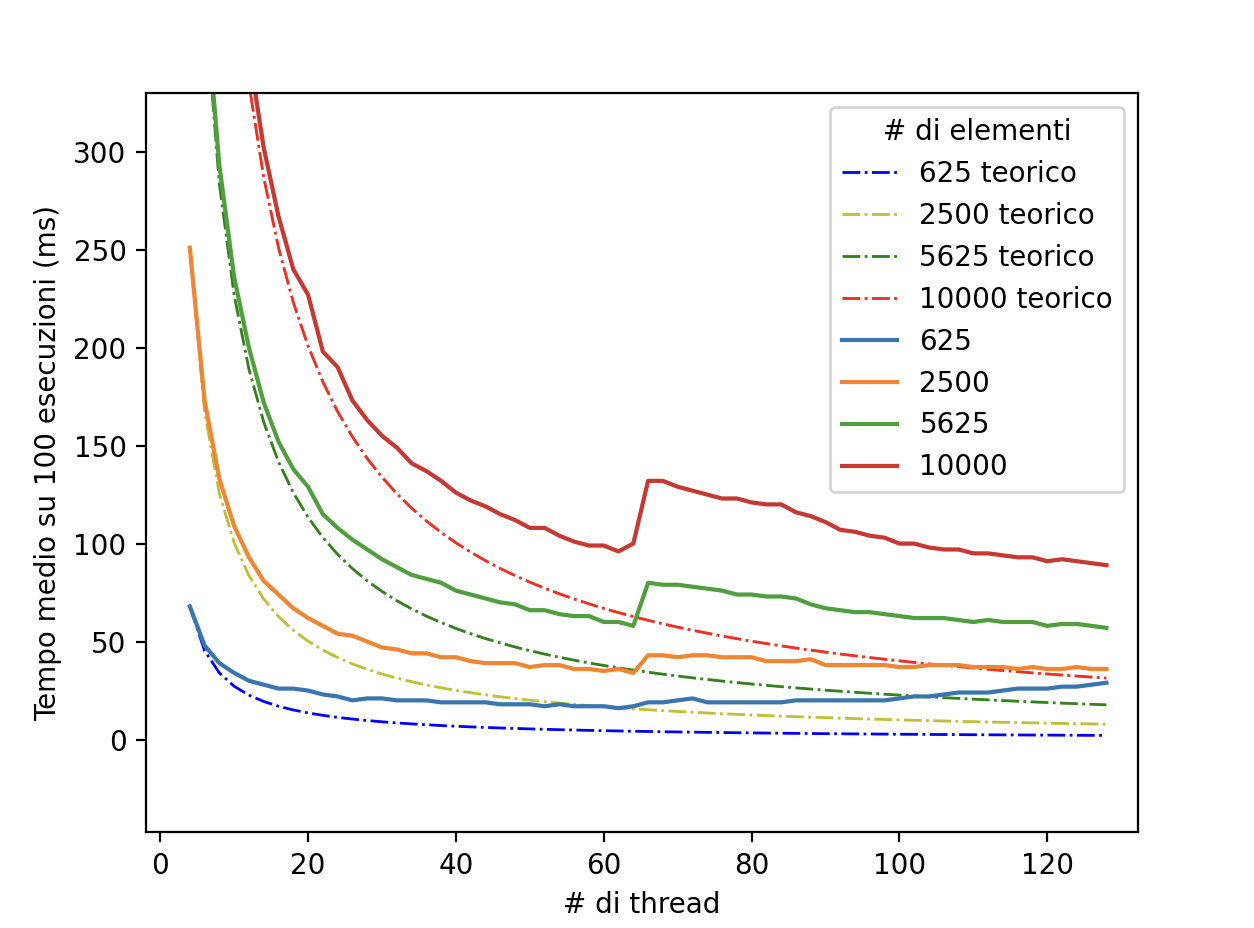
\includegraphics[width=8cm]{images/results/comp-threads.png}
    \caption{Comparazione performance tra diverso numero di thread}
    \label{fig:risultati-cpu}
  \end{minipage}
  \begin{minipage}[t]{0.5\linewidth}
    \centering
    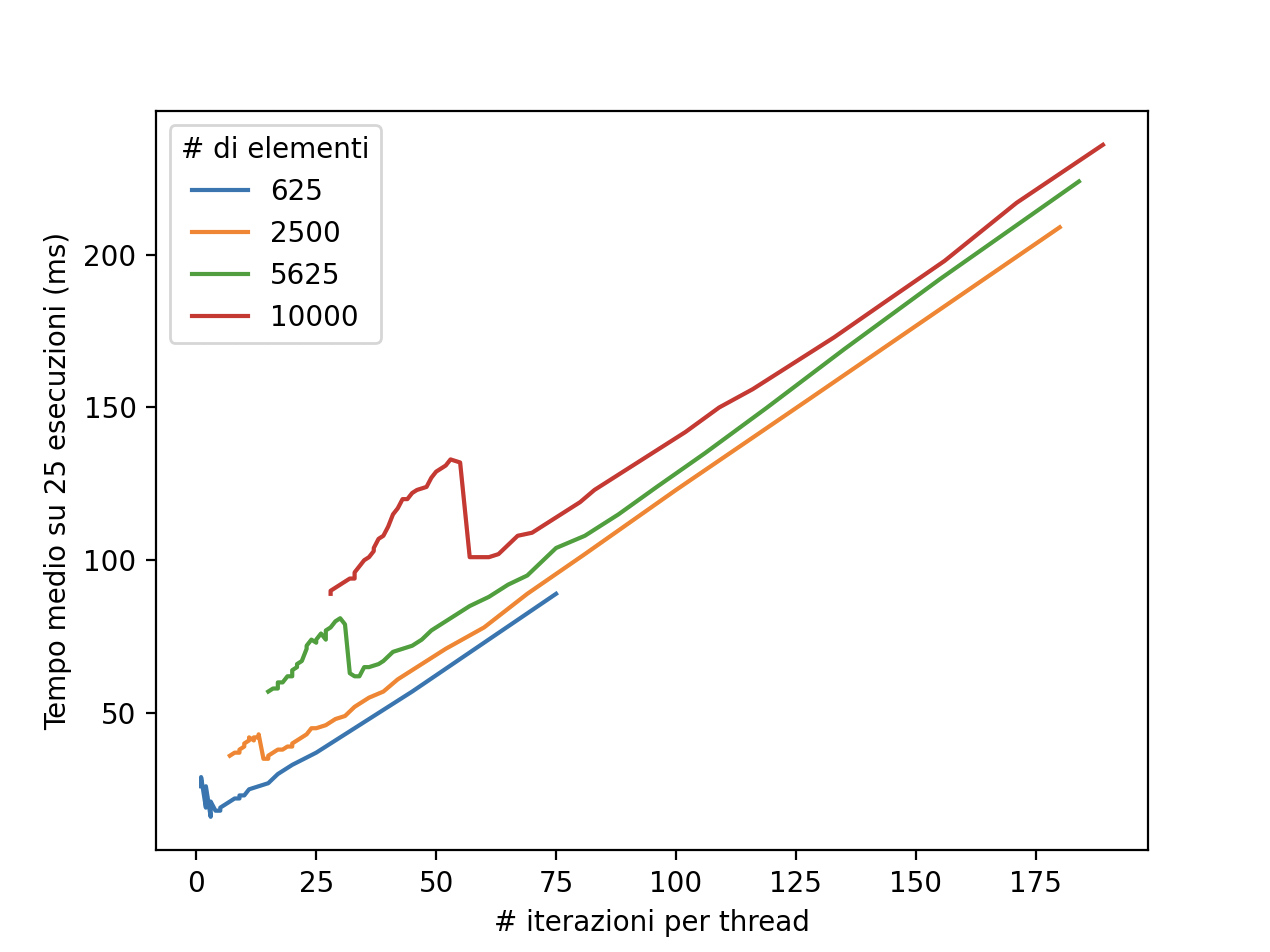
\includegraphics[width=8cm]{images/results/jobs-per-thread.png}
    \caption{Comparazione per grandezza di dati da computare per thread}
    \label{fig:jobs-per-thread}
  \end{minipage}
\end{figure}

\subsection{Risultati: Cuda vs OpenCL}
\label{subsec:risultati-cuda-opencl}

\lipsum[1]

\section{Dimostrazione sul framework}
\label{sec:dimostrazione}

\lipsum[1]